\section{СОКЕТ В ФАЙЛОВОМ ПРОСТРАНСТВЕ}

\begin{lstlisting}[caption=Функия error]
int error()
{
    fprintf(stderr, "%s\n", strerror(errno));
    return errno;
}
\end{lstlisting}

Сокеты в файловом пространстве используют в качестве адреса имя файла. В данной программе сервер создает сокет при помощи функции {\ttfamily socket} (с параметрами {\ttfamily AF\_UNIX}, что означает, что сокет будет в файловом пространстве, и {\ttfamily SOCK\_DGRAM}, что означает, что сокет будет датараммным) и связывает его с файлом {\ttfamily socket.soc} при помощи функции {\ttfamily bind}. После этого можно получать сообщения от клиентов при помощи функции {\ttfamily recvfrom}.

\begin{lstlisting}[caption=Текст программы сервера]
#include <string.h>
#include <sys/types.h>
#include <sys/socket.h>
#include <signal.h>
#include <stdlib.h>
#include <unistd.h>
#include "error.h"

#define SOCK_NAME "socket.soc"
#define SIZE_BUFFER 100
int sockfd;

void close_app()
{
    if (close(sockfd) < 0)
        exit(error());

    if (unlink(SOCK_NAME) < 0)
        exit(error());

    printf("\nSocket closed\n");
    exit(0);
}

int main()
{
    struct sockaddr socket_file;
    struct sockaddr recv_name;
    socklen_t recv_len;
    char buffer[SIZE_BUFFER];
    ssize_t size;

    signal(SIGINT, close_app);

    sockfd = socket(AF_UNIX, SOCK_DGRAM, 0);

    if (sockfd < 0)
        return error();

    socket_file.sa_family = AF_UNIX;
    strcpy(socket_file.sa_data, SOCK_NAME);

    bind(
        sockfd, &socket_file,
        strlen(socket_file.sa_data) + sizeof(socket_file.sa_family) + 1
    );

    if (errno != 0)
        return error();

    printf("Socket is successfully opened\n");
    printf("Press Ctrl+C to close this application\n");

    while (1)
    {
        size = recvfrom(
            sockfd, buffer, sizeof(buffer), 0,
            &recv_name, &recv_len
        );

        if (size < 0)
            return error();

        buffer[size] = '\0';
        printf("MESSAGE RECIEVED: %s", buffer);
    }

    return 0;
}
\end{lstlisting}

Клиент создает сокет с такими же параметрами, как и сервер, после чего задает тип домена и имя файла в структуру {\ttfamily sockaddr}, с помощью которой и отправляе соощение серверу фукцией {\ttfamily sendto}.

\begin{lstlisting}[caption=Текст программы клиента]
#include <sys/types.h>
#include <sys/socket.h>
#include <unistd.h>
#include <signal.h>
#include <stdlib.h>
#include "error.h"

#define SIZE_BUFFER 100

int sockfd;

void close_app()
{
    if (close(sockfd) < 0)
        exit(error());

    exit(0);
}

int main()
{
    size_t len;
    struct sockaddr srvr_name;
    char *buffer;

    signal(SIGINT, close_app);

    sockfd = socket(AF_UNIX, SOCK_DGRAM, 0);

    if (sockfd < 0)
        return error();

    srvr_name.sa_family = AF_UNIX;
    strcpy(srvr_name.sa_data, "socket.soc");

    while(1)
    {
        printf("Type message: ");
        getline(&buffer, &len, stdin);
        sendto(
            sockfd, buffer, strlen(buffer), 0, &srvr_name,
            strlen(srvr_name.sa_data) + sizeof(srvr_name.sa_family) + 1
        );
    }

    return 0;
}
\end{lstlisting}

\begin{figure}[H]
    \centering
    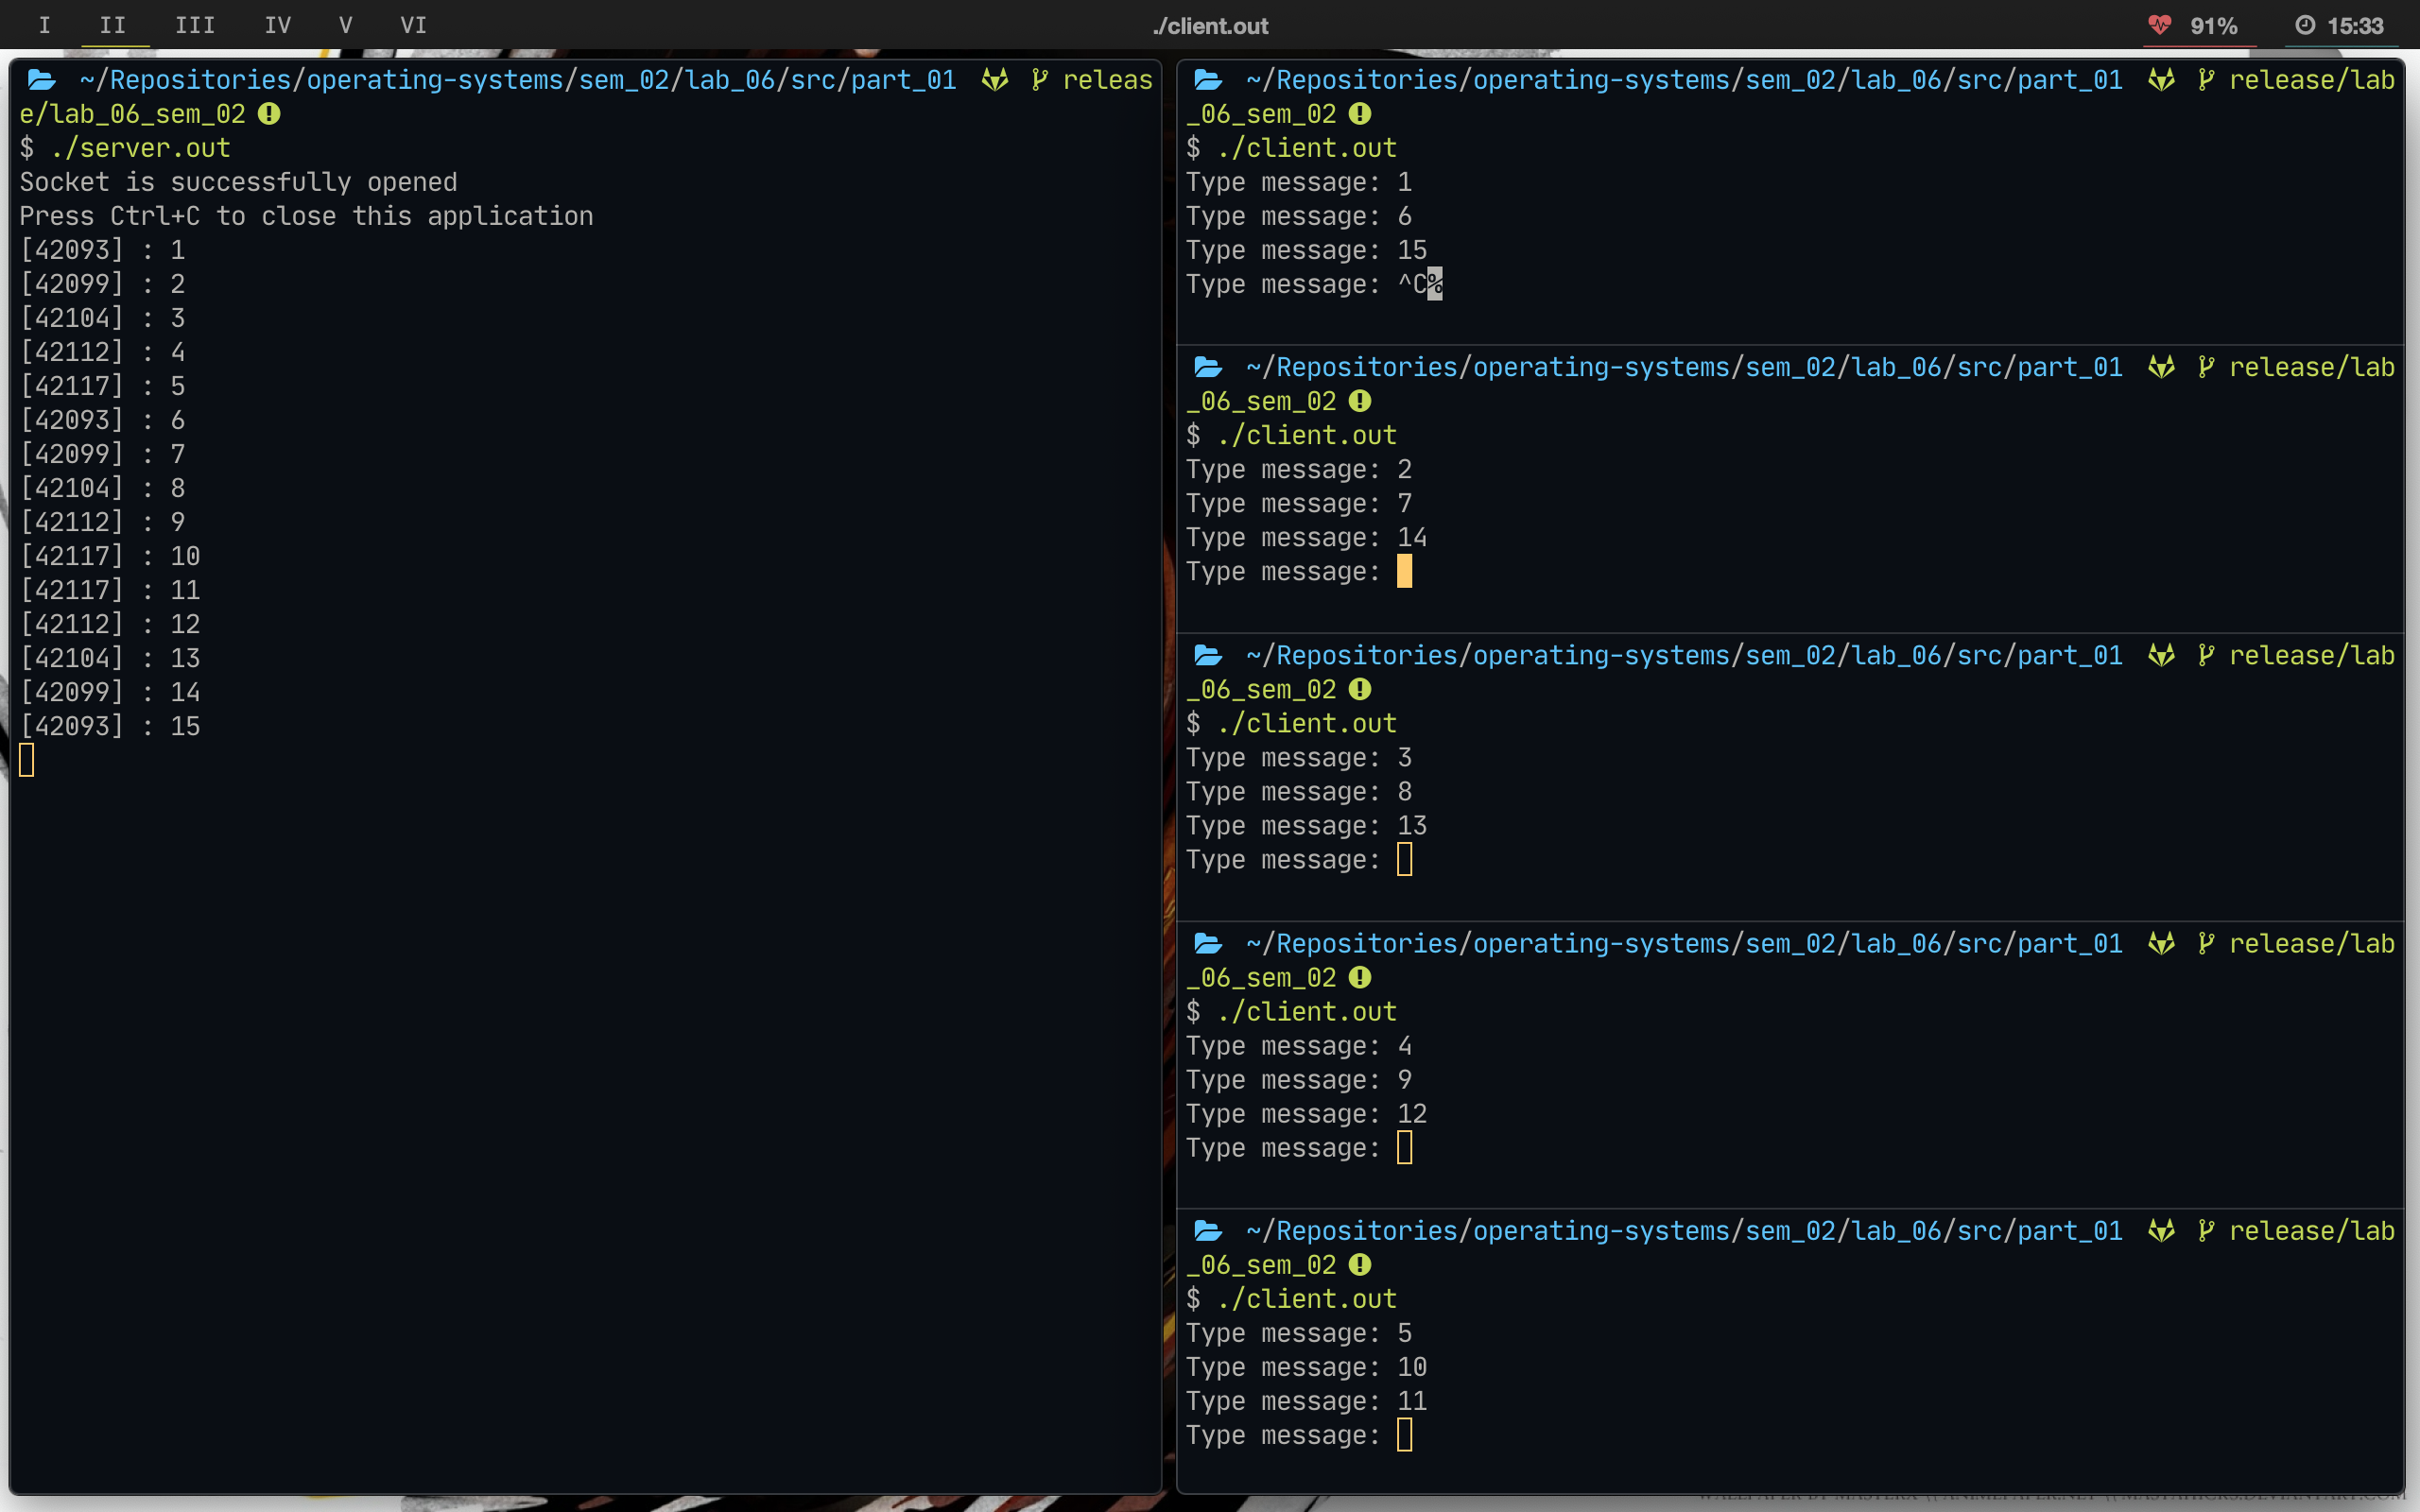
\includegraphics[scale=0.4]{img/file_socket.png}
    \caption{Результат работы программы}
\end{figure}

\section{СЕТЕВОЙ СОКЕТ}

Сервер создает сокет с параметрами {\ttfamily AF\_INET} (сетевое соединение) и {\ttfamily SOCK\_STREAM} (потоковый сокет). С помощью функции {\ttfamily bind} сокет связывается с адресом. После этого используется функция {\ttfamily listen}, которая переводит сервер в режим ожидания запроса на соединение. Затем создается массив дескрипторов для будущих подключаемых клиентов. Если дескриптор равен -1, то значит он свободен для новых клиентов. После проделанных действий можно ожидать подключения от клиентов. В функции {\ttfamily connection}, которая служит в этой программе для подключения новых клиентов, с помощью функции {\ttfamily accept} устанавливается соединение, затем находим свободный элемент в массиве дескрипторов и добавляем нового клиента, получив от него первое сообщение, содержащее его pid. Функция {\ttfamily message} принимает сообщения от подключенных клиентов и проверяет на отключение от сервера. В этой функции производится проверка дескрипторов всех подключенных клиентов. Если появляется возможность чтения или записи из дескриптора, то происходит провера на соединение с клиентом. Если соединения нет, то освобождается дескриптор и выводится сообщение об отключении клиента. В ином случае выводится полученное сообщение и отправляется ответное.

\begin{lstlisting}[caption=Текст программы сервера]
#include <sys/types.h>
#include <sys/socket.h>
#include <unistd.h>
#include <stdlib.h>
#include <strings.h>
#include <netinet/in.h>
#include <signal.h>
#include "error.h"

#define SIZE_BUFFER 100
#define CLIENTS 100

int sockfd;
int maxi, maxfd;
int pid_client[CLIENTS];

void close_signal()
{
    if (close(sockfd) < 0)
        exit(error());

    printf("\nSocket closed\n");
    exit(0);
}

int connection(int client[FD_SETSIZE], fd_set *allset, fd_set *rset)
{
    int i;
    int connfd;
    int message_len;
    char buffer[SIZE_BUFFER];

    if (FD_ISSET(sockfd, rset))
    {
        connfd = accept(sockfd, NULL, NULL);

        if (connfd < 0)
            return errno;

        for (i = 0; i < FD_SETSIZE; i++)
        {
            if (client[i] < 0)
            {
                client[i] = connfd;
                break;
            }
        }

        if (i == FD_SETSIZE)
            return errno;

        FD_SET(connfd, allset);

        if (connfd > maxfd)
            maxfd = connfd;

        if (i > maxi)
            maxi = i;

        message_len = read(connfd, buffer, SIZE_BUFFER);
        pid_client[i] = atoi(buffer);
        printf("[%d] connected\n", pid_client[i]);
    }

    return 0;
}

int message(int client[FD_SETSIZE], fd_set *allset, fd_set *rset)
{
    int n, i;
    int sockfd;
    char buffer[SIZE_BUFFER];

    for (i = 0; i <= maxi; i++)
    {
        sockfd = client[i];
        if (sockfd > 0)
        {
            if (FD_ISSET(sockfd, rset))
            {
                n = read(sockfd, buffer, SIZE_BUFFER);

                if (n == 0)
                {
                    close(sockfd);
                    FD_CLR(sockfd, allset);
                    client[i] = -1;
                    printf("[%d] disconnected\n", pid_client[i]);
                }
                else
                {
                    write(sockfd, "good", 4);
                    printf("[%d] : %s", pid_client[i], buffer);
                }
            }
        }
    }

    return 0;
}

int main(int argc, char **argv)
{
    if (argc != 2)
    {
        fprintf(stderr, "Usage: %s <port>\n", argv[0]);
        return -1;
    }

    int client[FD_SETSIZE];
    fd_set rset;
    fd_set allset;
    struct sockaddr_in server;

    signal(SIGINT, close_signal);

    sockfd = socket(AF_INET, SOCK_STREAM, 0);

    if (sockfd < 0)
        return errno;

    server.sin_family = AF_INET;
    server.sin_addr.s_addr = INADDR_ANY;
    server.sin_port = htons(atoi(argv[1]));

    bind(sockfd, (struct sockaddr *) &server, sizeof(server));

    if (errno != 0)
        return errno;

    listen(sockfd, CLIENTS);

    maxfd = sockfd;
    maxi = -1;

    for (int i = 0; i < FD_SETSIZE; i++)
        client[i] = -1;

    FD_ZERO(&allset);
    FD_SET(sockfd, &allset);

    printf("Socket is successfully opened\n");
    printf("Press Ctrl+C to close this application\n");

    while(1)
    {
        rset = allset;
        select(maxfd + 1, &rset, NULL, NULL, NULL);

        connection(client, &allset, &rset);

        if (errno != 0)
            return error();

        message(client, &allset, &rset);

        if (errno != 0)
            return error();
    }

    return 0;
}
\end{lstlisting}

Клиент создает сокет с теми же параметрами, как и сервер. После этого, клиенту необходимо подключиться по адресу. Это делается с помощью структуры {\ttfamily sockaddr\_in}, поля которой необходимо заполнить информацией о сервере, к которому мы хотим подключиться. Функцией {\ttfamily connect} производится подключение. После успешного подключения, клиент отправляет свой pid сообщением и начинает отправлять сообщения, введенные пользователем. После каждого отправленного сообщения клиент ждет ответного сообщения от сервера. Отправка сообщения производится функцией {\ttfamily write}, получение -- {\ttfamily read}.

\begin{lstlisting}[caption=Текст программы клиента]
#include <stdint.h>
#include <stdio.h>
#include <sys/types.h>
#include <sys/socket.h>
#include <unistd.h>
#include <netinet/in.h>
#include <netdb.h>
#include <stdlib.h>
#include <signal.h>
#include "error.h"

#define SIZE_BUFFER 100

int sockfd;

void close_signal()
{
    if (close(sockfd) < 0)
        exit(error());

    printf("\nSocket closed\n");
    exit(0);
}

int main(int argc, char *argv[])
{
    if (argc != 3)
    {
        printf("Usage: %s <servername> <port>", argv[0]);
        return -1;
    }

    signal(SIGINT, close_signal);

    struct hostent *server;
    struct sockaddr_in serv_addr;
    char *buffer = NULL;
    size_t len;
    char buffer_server[SIZE_BUFFER];

    sockfd = socket(AF_INET, SOCK_STREAM, 0);

    if (sockfd < 0)
        return error();

    server = gethostbyname(argv[1]);

    if (server == NULL)
        return error();

    serv_addr.sin_family = AF_INET;
    strncpy(
        (char *)&serv_addr.sin_addr.s_addr,
        (char *)server->h_addr, server->h_length
    );
    serv_addr.sin_port = htons(atoi(argv[2]));

    connect(sockfd, (struct sockaddr *)&serv_addr, sizeof(serv_addr));

    if (errno != 0)
        return error();

    buffer = calloc(10, 1);
    sprintf(buffer, "%d", getpid());
    write(sockfd, buffer, strlen(buffer));

    free(buffer);
    buffer = NULL;

    printf("Type message: ");
    getline(&buffer, &len, stdin);
    buffer[len] = '\0';

    while (strcmp(buffer, "exit\n"))
    {
        write(sockfd, buffer, len);

        memset(buffer_server, 0, SIZE_BUFFER);
        read(sockfd, buffer_server, SIZE_BUFFER);
        printf("Message received: %s\n", buffer_server);

        printf("Type message: ");
        getline(&buffer, &len, stdin);
        buffer[len] = '\0';
    }

    return 0;
}
\end{lstlisting}

\begin{figure}[H]
    \centering
    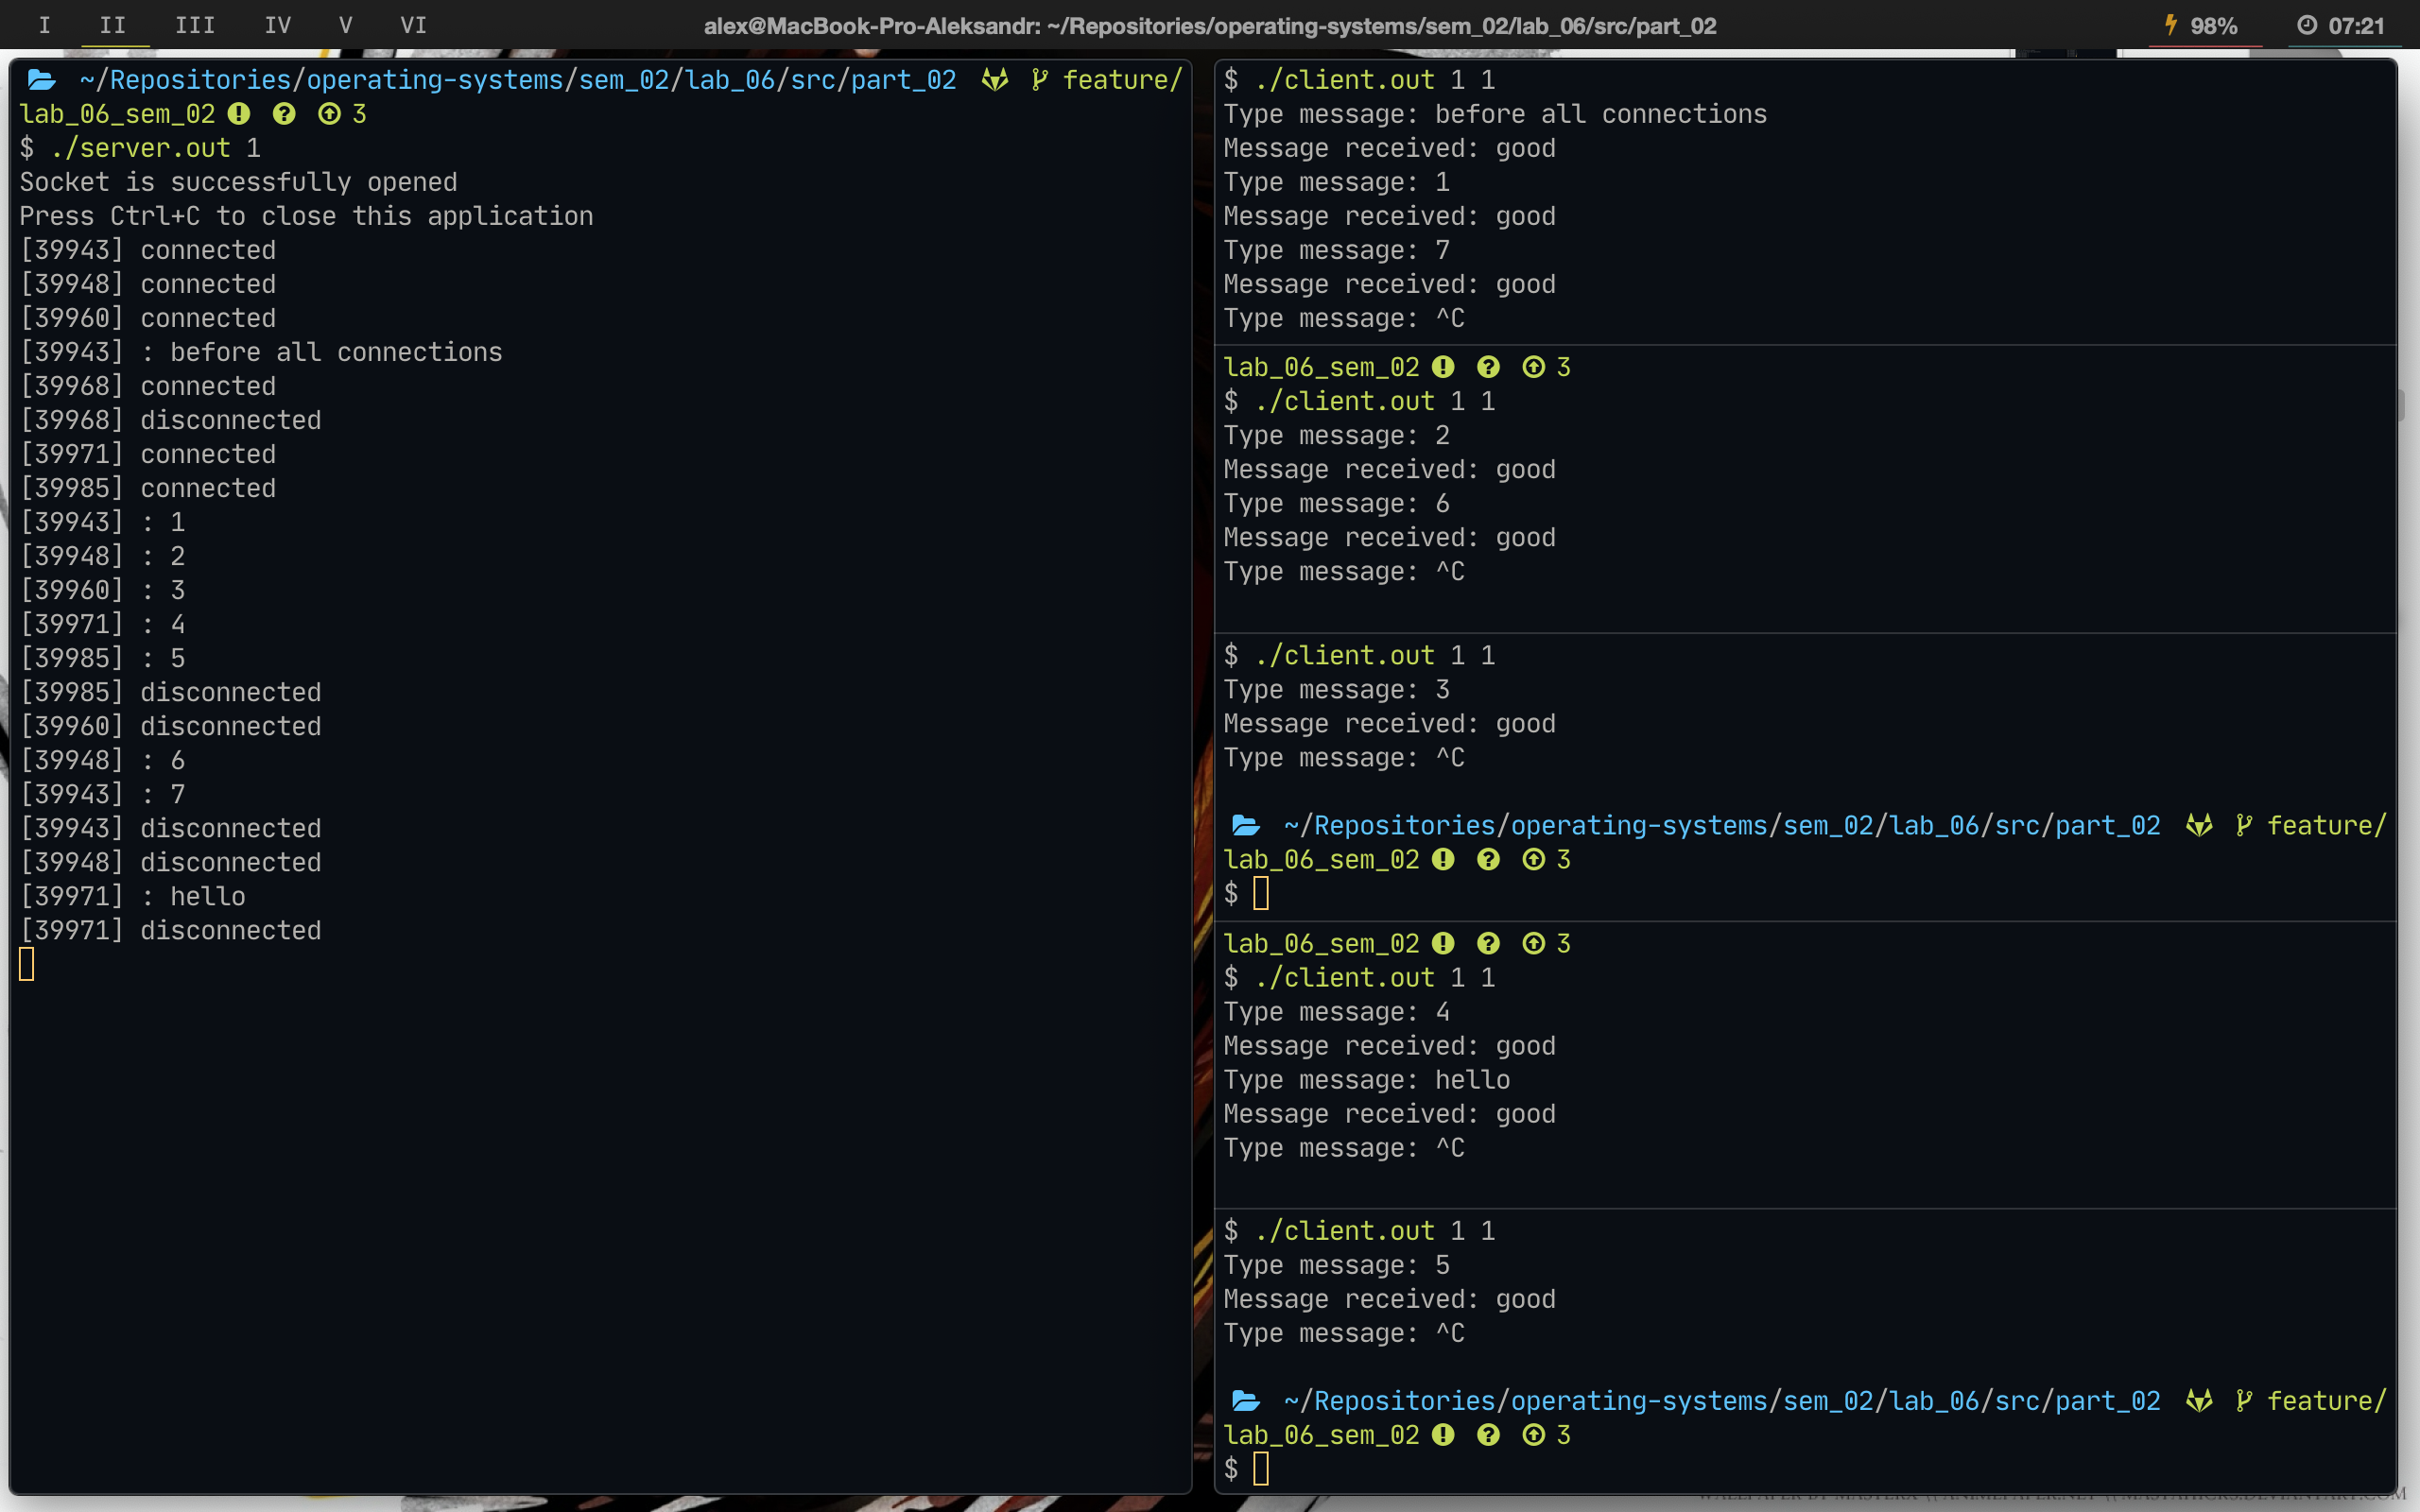
\includegraphics[scale=0.4]{img/inet_socket.png}
    \caption{Результат работы программы}
\end{figure}
